\chapter{基礎知識}
本章では,本論文で扱うProgrammable Microfluidic Device(PMD)\mout{と呼ばれる}バイオチップの基礎知識について説明をする.
まず,PMDのアーキテクチャについて説明する.
\mout{その後},PMDのアーキテクチャの欠点についても説明する.
最後に,既存手法として,PMDのアーキテクチャの欠点に対応したPMD上での混合手順の生成手法
No Transport Mixing(NTM)について簡単に説明する.
\section{PMD}
\label{PMD}
本節では,PMDのアーキテクチャがどういった特徴や欠点を持つかを説明する.
\subsection{PMDのアーキテクチャ}
\label{arc}
%PMDとはどういうデバイスか説明を書く.
PMDの顕微鏡写真を図~\ref{fig:micrograph}に示\cout{す}~\cite{1}.
図~\ref{fig:micrograph}において,赤黒く見えるのはバルブと\mout{呼ばれる}部品で,バルブによって囲まれていて青い線の交点と重なっている領域はセルと呼ばれる.
バルブは開閉の操作を行うことが可能である.
図~\ref{fig:mixing}は,PMD上に流し込まれた2種類の試薬が混合される様子を\cout{示}している~\cite{4}.
図~\ref{fig:mixing}(a)から(b)は,圧力をかけられることで試薬が入力ポートからPMDの内部へと流し込まれる様子を\cout{示}している.
図~\ref{fig:mixing}(c)は,バルブの開閉の制御によって,ミキサーと呼ばれる,セルが円環状に繋げられた流路が生成される様子を\cout{示}している.
ミキサー内のバルブの開閉を行うことにより,ミキサー内の液滴の混合が行われる.
液滴の混合後は,図~\ref{fig:mixing}(d)で\cout{示}されているようにミキサー内のどのセルにおいても格納されている液滴の濃度は等しくなる.

また,PMDでは,図~\ref{fig:4and6Mixer}で\cout{示}したよう\mout{に}様々な大きさのミキサーを生成すること\mout{が}できる.
図~\ref{fig:4and6Mixer}(a)は2$\times2$のセルを用いる2$\times2$ミキサー,図~\ref{fig:4and6Mixer}(b)は2$\times$3セルを用いる2$\times$3ミキサーである.
\cout{PMDでは,}これら以外にも様々な大きさのミキサーの生成,及び,そのミキサー上での試薬の混合が可能である.
\begin{figure}[tbp]
 \centering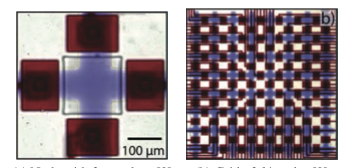
\includegraphics[scale=1.2]{img/PMDMicrograph.pdf}
 \caption{PMDの顕微鏡写真,参考文献~\cite{1}より引用}\label{fig:micrograph}
\end{figure}
\begin{figure}[tbp]
 \centering\includegraphics[scale=1.0]{img/PMDMixing_jp.pdf}
    \caption{PMD上に流し込まれた2種類の試薬が混合される様子,参考文献~\cite{4}より引用し一部改変}\label{fig:mixing}
\end{figure}
\begin{figure}[tbp]
    \centering\includegraphics[scale=0.5]{img/Modified_4and6Mixer.pdf}
 \caption{PMDで生成可能なミキサー}\label{fig:4and6Mixer}
\end{figure}
\newpage
\subsection{PMDにおけるセル間の液滴の移動}
%既存手法の説明への前提知識として,PMDにおいてセル間での液滴の移動操作は原則不可能であるということを説明する.
バイオチップの中心的なアーキテクチャであるDMFB(Digital Microfluid biochip)においては,PMDでのセルに相当する電極の間での液滴の移動操作~\cite{B110474H}を用い,試薬合成が行われる~\cite{5605330}\cite{10.1007/s11047-006-9032-6}\cite{10.1145/2429384.2429464}.
それに対して,PMDでは,セル間での液滴の移動操作は原則不可能であることが知られている.
図~\ref{fig:fluidseg}は\mout{,Flow-based Microfluidic Biochip(FMB)と呼ばれるバイオチップにおいて一般的に使用される液体の移動操作の手法を応用し,PMD上での試薬液滴の移動操作を試みたものの,失敗した際の様子を示している}~\cite{4}. 

\mout{この試薬液滴の移動操作の手法は,試薬液滴と油は混じり合わないという特性を利用し,油に試薬液滴を乗せた液体に圧力をかけることで試薬液滴を移動させる.
\mout{また,}移動経路上の届け先セルのところには油のみを通すマイクロ流体ラッチと呼ばれる特殊なバルブを備え付けておく.
これにより,届け先セル上に試薬液滴のみが濾し取られ,試薬液滴の移動操作が実行されるというものである.}
図~\ref{fig:fluidseg}(a)は,始点セルから届け先セルへの\cout{試薬}液滴の移動操作を試みる前の状態を\cout{示している.}
\mout{また,}図~\ref{fig:fluidseg}(b)は,油のみを通すマイクロ流体ラッチ~\cite{urbanski2006digital}と油を用いて始点セルから届け先セルへの試薬液滴の移動操作を試みた後の様子\cout{を示している}.
\mout{図~\ref{fig:fluidseg}(b)では,油に試薬液滴を載せた液体の移動経路上において試薬液滴の分割が発生している~\cite{FU2015343}.}
\mout{これは,油に試薬液滴を載せた液体の移動経路上の直角のところで\cout{試薬}液滴にかかる力が,部分ごとに均一でなくなるからである.}

以上で述べたように,経路上において液滴の分割が発生するため,PMDにおけるセル間の液滴の移動操作は不可能である.
したがって,PMDで試薬合成を行うためには,セル間での液滴移動のない混合手順を生成する必要がある.
\begin{figure}[tbp]
    \centering\includegraphics[scale=0.9]{img/FluidSegmentation.pdf}
 \caption{fluid segmentationの様子,参考文献~\cite{4}より引用し一部改変}\label{fig:fluidseg}
\end{figure}
\newpage
\section{{2×2ミキサーを用いた液滴移動の\bout{ない}混合手順の生成}}
%セル間の液滴の移動操作を必要としない試薬混合手法NTM(No Transport Mixing)の説明をする.
%その後,既存の希釈木のNTMでのPMDへのマッピング手法を説明する.
\ref{arc}~節で述べた通り,PMDで試薬合成を行うためには,セル間での液滴移動のない混合手順を生成する必要がある.
したがって,本節では既存のPMD上でのセル間の液滴移動のない混合手順の生成手法NTM(No Transport Mixing)の説明をする.
図~\ref{fig:ntmresult}はNTMの入出力データを\cout{示}している~\cite{4}.
NTMは,図~\ref{fig:ntmresult}(a)\cout{が示し}ているような希釈木を入力として受け取り,図~\ref{fig:ntmresult}(b)から(e)
\cout{が示し}ているような,希釈木に対応したPMD上での液滴の移動のない混合手順を生成する.
希釈木とは,試薬合成で目標濃度の\cout{混合}液滴を得るために,\cout{液滴の混合をどのように行えば良いか}を木で表したものである.
図~\ref{fig:ntmresult}(a)の希釈木において,ミキサーでの液滴の混合はM1からM4のミキサーノードで表され,
\mout{ミキサーでの液滴の混合で用いられる}試薬液滴は,\mout{希釈木の葉に位置する}試薬\mout{液滴}ノードで表されている.
また,図~\ref{fig:ntmresult}(a)の希釈木のエッジに付加された重みは,親ミキサーノードが\mout{子ミキサーノード,もしくは,子試薬液滴ノード}から受け取る液滴の数を表している.

\ref{arc}~節で述べたように,PMDは2$\times$3ミキサーなど,2$\times$2以外の大きさを持つミキサーを生成できる.
しかし,本節で紹介してきたNTMには,2$\times$2ミキサーノードのみを含む希釈木しか扱うことができないという制約がある.
この制約のために,NTMが扱うことのできる希釈木の種類は大きく制限されている.
したがって,PMD上の液滴移動のない混合手順の生成手法には,NTMより多くの種類の希釈木を扱うことが出来るように拡張する余地がある.
NTMでは扱えなかった希釈木を扱えるようになれば,手法としての汎用性は高まる.
\begin{figure}[tbp]
 \centering\includegraphics[scale=0.7]{img/NTMResult_jp.pdf}
    \caption{NTMの入力データと出力データ,参考文献~\cite{4}より引用し一部改変}\label{fig:ntmresult}
\end{figure}

